\documentclass{standalone}

\usepackage{tikz}
\usetikzlibrary{calc}
\usetikzlibrary{decorations}
\usetikzlibrary{decorations.markings}

\begin{document}
  %noformat{
  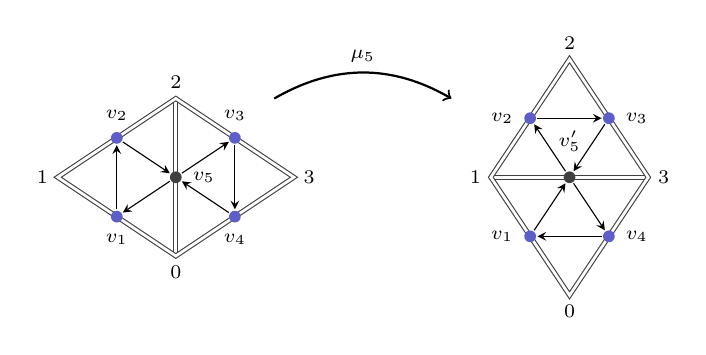
\begin{tikzpicture}
    \tikzstyle{v1} = [circle, outer sep=0.5pt, fill, inner sep=1.5pt]
    \tikzstyle{v2} = [circle, outer sep=0.5pt, fill, inner sep=3.0pt]
    \tikzstyle{unf} = [color=darkgray]
    \tikzstyle{frz} = [color=blue!60!darkgray!70]
    \tikzstyle{r} = [color=red!70!darkgray!70]
    \tikzstyle{e} = [->, >={stealth}, preaction={draw=white, -, ultra thick}]
    \tikzstyle{b} = [fill, fill opacity=0.0, circle, outer sep=0.5pt, inner sep=1.5pt]
    \tikzstyle{te} = [color=darkgray, double distance=1pt]
    \tikzstyle{h} = [dashed, color=gray, ->, >={stealth}]
    \tikzstyle{se} = [postaction=decorate, decoration={markings, mark=at position 0.9 with {\arrow{stealth}}}]

    \tikzset{font=\scriptsize}

    \begin{scope}[shift={(0,0)}]
      % Copied from fig-dv-construction.tex
      \coordinate[label=270:{$0$}] (q_0) at (270:1.0);
      \coordinate[label=180:{$1$}] (q_1) at (180:1.5);
      \coordinate[label= 90:{$2$}] (q_2) at ( 90:1.0);
      \coordinate[label=  0:{$3$}] (q_3) at (  0:1.5);

      \draw[te] (q_0) -- (q_2);
      \draw[te] (q_0) -- (q_1) -- (q_2) -- (q_3) -- cycle;
 
      \node[v1, frz, label={270:{$v_{1}$}}] (D1) at    ($ (q_0)!0.50!(q_1) $) {};
      \node[v1, frz, label={ 90:{$v_{2}$}}] (E1) at    ($ (q_1)!0.50!(q_2) $) {};
      \node[v1, frz, label={ 90:{$v_{3}$}}] (F1) at    ($ (q_2)!0.50!(q_3) $) {};
      \node[v1, frz, label={270:{$v_{4}$}}] (G1) at    ($ (q_0)!0.50!(q_3) $) {};

      \node[v1, unf, label={  0:{$v_{5}$}}] (w11) at ($ (q_0)!0.50!(q_2) $) {};

      \draw[e] (D1) -- (E1);
      \draw[e] (E1) -- (w11);
      \draw[e] (w11) -- (D1);

      \draw[e] (F1) -- (G1);
      \draw[e] (G1) -- (w11);
      \draw[e] (w11) -- (F1);
    \end{scope}


    \begin{scope}[shift={(5,0)}]
      \coordinate[label=270:{$0$}] (q_0) at (270:1.5);
      \coordinate[label=180:{$1$}] (q_1) at (180:1.0);
      \coordinate[label= 90:{$2$}] (q_2) at ( 90:1.5);
      \coordinate[label=  0:{$3$}] (q_3) at (  0:1.0);

      \draw[te] (q_1) -- (q_3);
      \draw[te] (q_0) -- (q_1) -- (q_2) -- (q_3) -- cycle;
 
      \node[v1, frz, label={180:{$v_{1}$}}] (D1) at    ($ (q_0)!0.50!(q_1) $) {};
      \node[v1, frz, label={180:{$v_{2}$}}] (E1) at    ($ (q_1)!0.50!(q_2) $) {};
      \node[v1, frz, label={  0:{$v_{3}$}}] (F1) at    ($ (q_2)!0.50!(q_3) $) {};
      \node[v1, frz, label={  0:{$v_{4}$}}] (G1) at    ($ (q_0)!0.50!(q_3) $) {};

      \node[v1, unf, label={[label distance=3pt] 90:{$v_{5}'$}}] (w11) at ($ (q_0)!0.50!(q_2) $) {};

      \draw[e] (E1) -- (F1);
      \draw[e] (F1) -- (w11);
      \draw[e] (w11) -- (E1);

      \draw[e] (G1) -- (D1);
      \draw[e] (D1) -- (w11);
      \draw[e] (w11) -- (G1);
    \end{scope}

    \draw[->, thick] ( 1.25, 1.0) to[bend left ] node[midway, above] (t01) {$\mu_{5}$} ( 3.5, 1.0);
  \end{tikzpicture}
  %}noformat
\end{document}
